\documentclass{article}
\usepackage[T1]{fontenc}
\usepackage[utf8]{inputenc}
\usepackage[margin=1in]{geometry}
\usepackage{fancyhdr} 
\usepackage{listings}
\usepackage[ruled,vlined]{algorithm2e}
\usepackage{amsthm}
\usepackage{amsfonts}
\usepackage{amssymb}
\usepackage{graphicx}
\usepackage[dvipsnames]{xcolor}
\usepackage{xy}
% \usepackage{url} % Commented out because hyperref provides similar functionality
\usepackage{parskip}
\usepackage{comment}
\usepackage{setspace}
\usepackage{enumerate}
\usepackage{multirow}
\usepackage{hyperref}
\usepackage{caption}
\usepackage{subcaption}
\usepackage{booktabs}
\usepackage{wrapfig}
\usepackage{times}

\captionsetup[figure]{font={small,it}}

\usepackage[backend=biber,style=numeric,sortcites,maxbibnames=99]{biblatex}
\addbibresource{references.bib}

\newcommand{\HRule}{\rule{\linewidth}{0.5mm}}
\newcommand{\Hrule}{\rule{\linewidth}{0.3mm}}
\newcommand{\classnum}{CS-GY 6313 B}

\makeatletter% since there's an at-sign (@) in the command name
\renewcommand{\@maketitle}{%
  \parindent=0pt% don't indent paragraphs in the title block
  \centering
  {\Large \bfseries\textsc{\@title}}
  \HRule\par%
  \textit{\@author \hfill \classnum}
  \par
}
\makeatother% resets the meaning of the at-sign (@)

\title{Assignment 3: Interactive Visualization} 
\author{Ivan Aristy — iae225}
% \classnum

\begin{document}
  \maketitle % prints the title block
  \thispagestyle{empty}
  % \vspace{-15pt}

\section{Interactive Visualization}
\label{sec:sec1}

\subsection{Question }
\label{subsec:subsec1}

\textbf{How has my champion's win rate changed over time? Is my champion still strong in the current meta?}

I want the user to easily see the win rate of their champion over time. 
Winrate is a key metric in League of Legends, as it is a good indicator of how strong a champion is in the current meta.
This would allow the user to see how their champion has been impacted in recent patches.

Winrate is not a direct representation of power, since some champions are harder to play than others.
Easy champions usually have high winrates, while hard champions have lower winrates.
Additionally, hyper-specific champions have really high winrates, since they are only played in specific situations.

Nevertheless, patterns in winrates can be indicative of power. For example, a 2\% growth in winrates
over a patch can be indicative of a very strong relating buff, while a 2\% decrease can be indicative of a strong relative nerf.
Additionally, a winrate that is consistently above 50\% can show that a champion has and is strong in the current meta.

\subsection{Data}
\label{subsec:subsec2}

\subsubsection{Data Source}
\label{subsubsec:Data Source}

Riot's Developer API is very hard to use. In my opinion, is not well documented, and it is very hard to get the data you want.
Hence, I wll scrape some data off the internet to get the winrate of a champion over time.

Particularly I need:
\begin{enumerate}
  \item The winrate of a champions over time.
  \item The tier of the champion over time.
  \item Visual Assets of the champion.
\end{enumerate}

\subsubsection{Data Retreival} 
\label{subsubsec:Data Retreival}

To get winrate data, I will scrape \url{https://lolalytics.com/lol/tierlist/} for the winrate and tier of a champion over time.

After analyzing the beautiful soup output, 


% \begin{figure}[ht] % Change the position of your figure https://www.overleaf.com/learn/latex/Positioning_images_and_tables
%   \centering
%   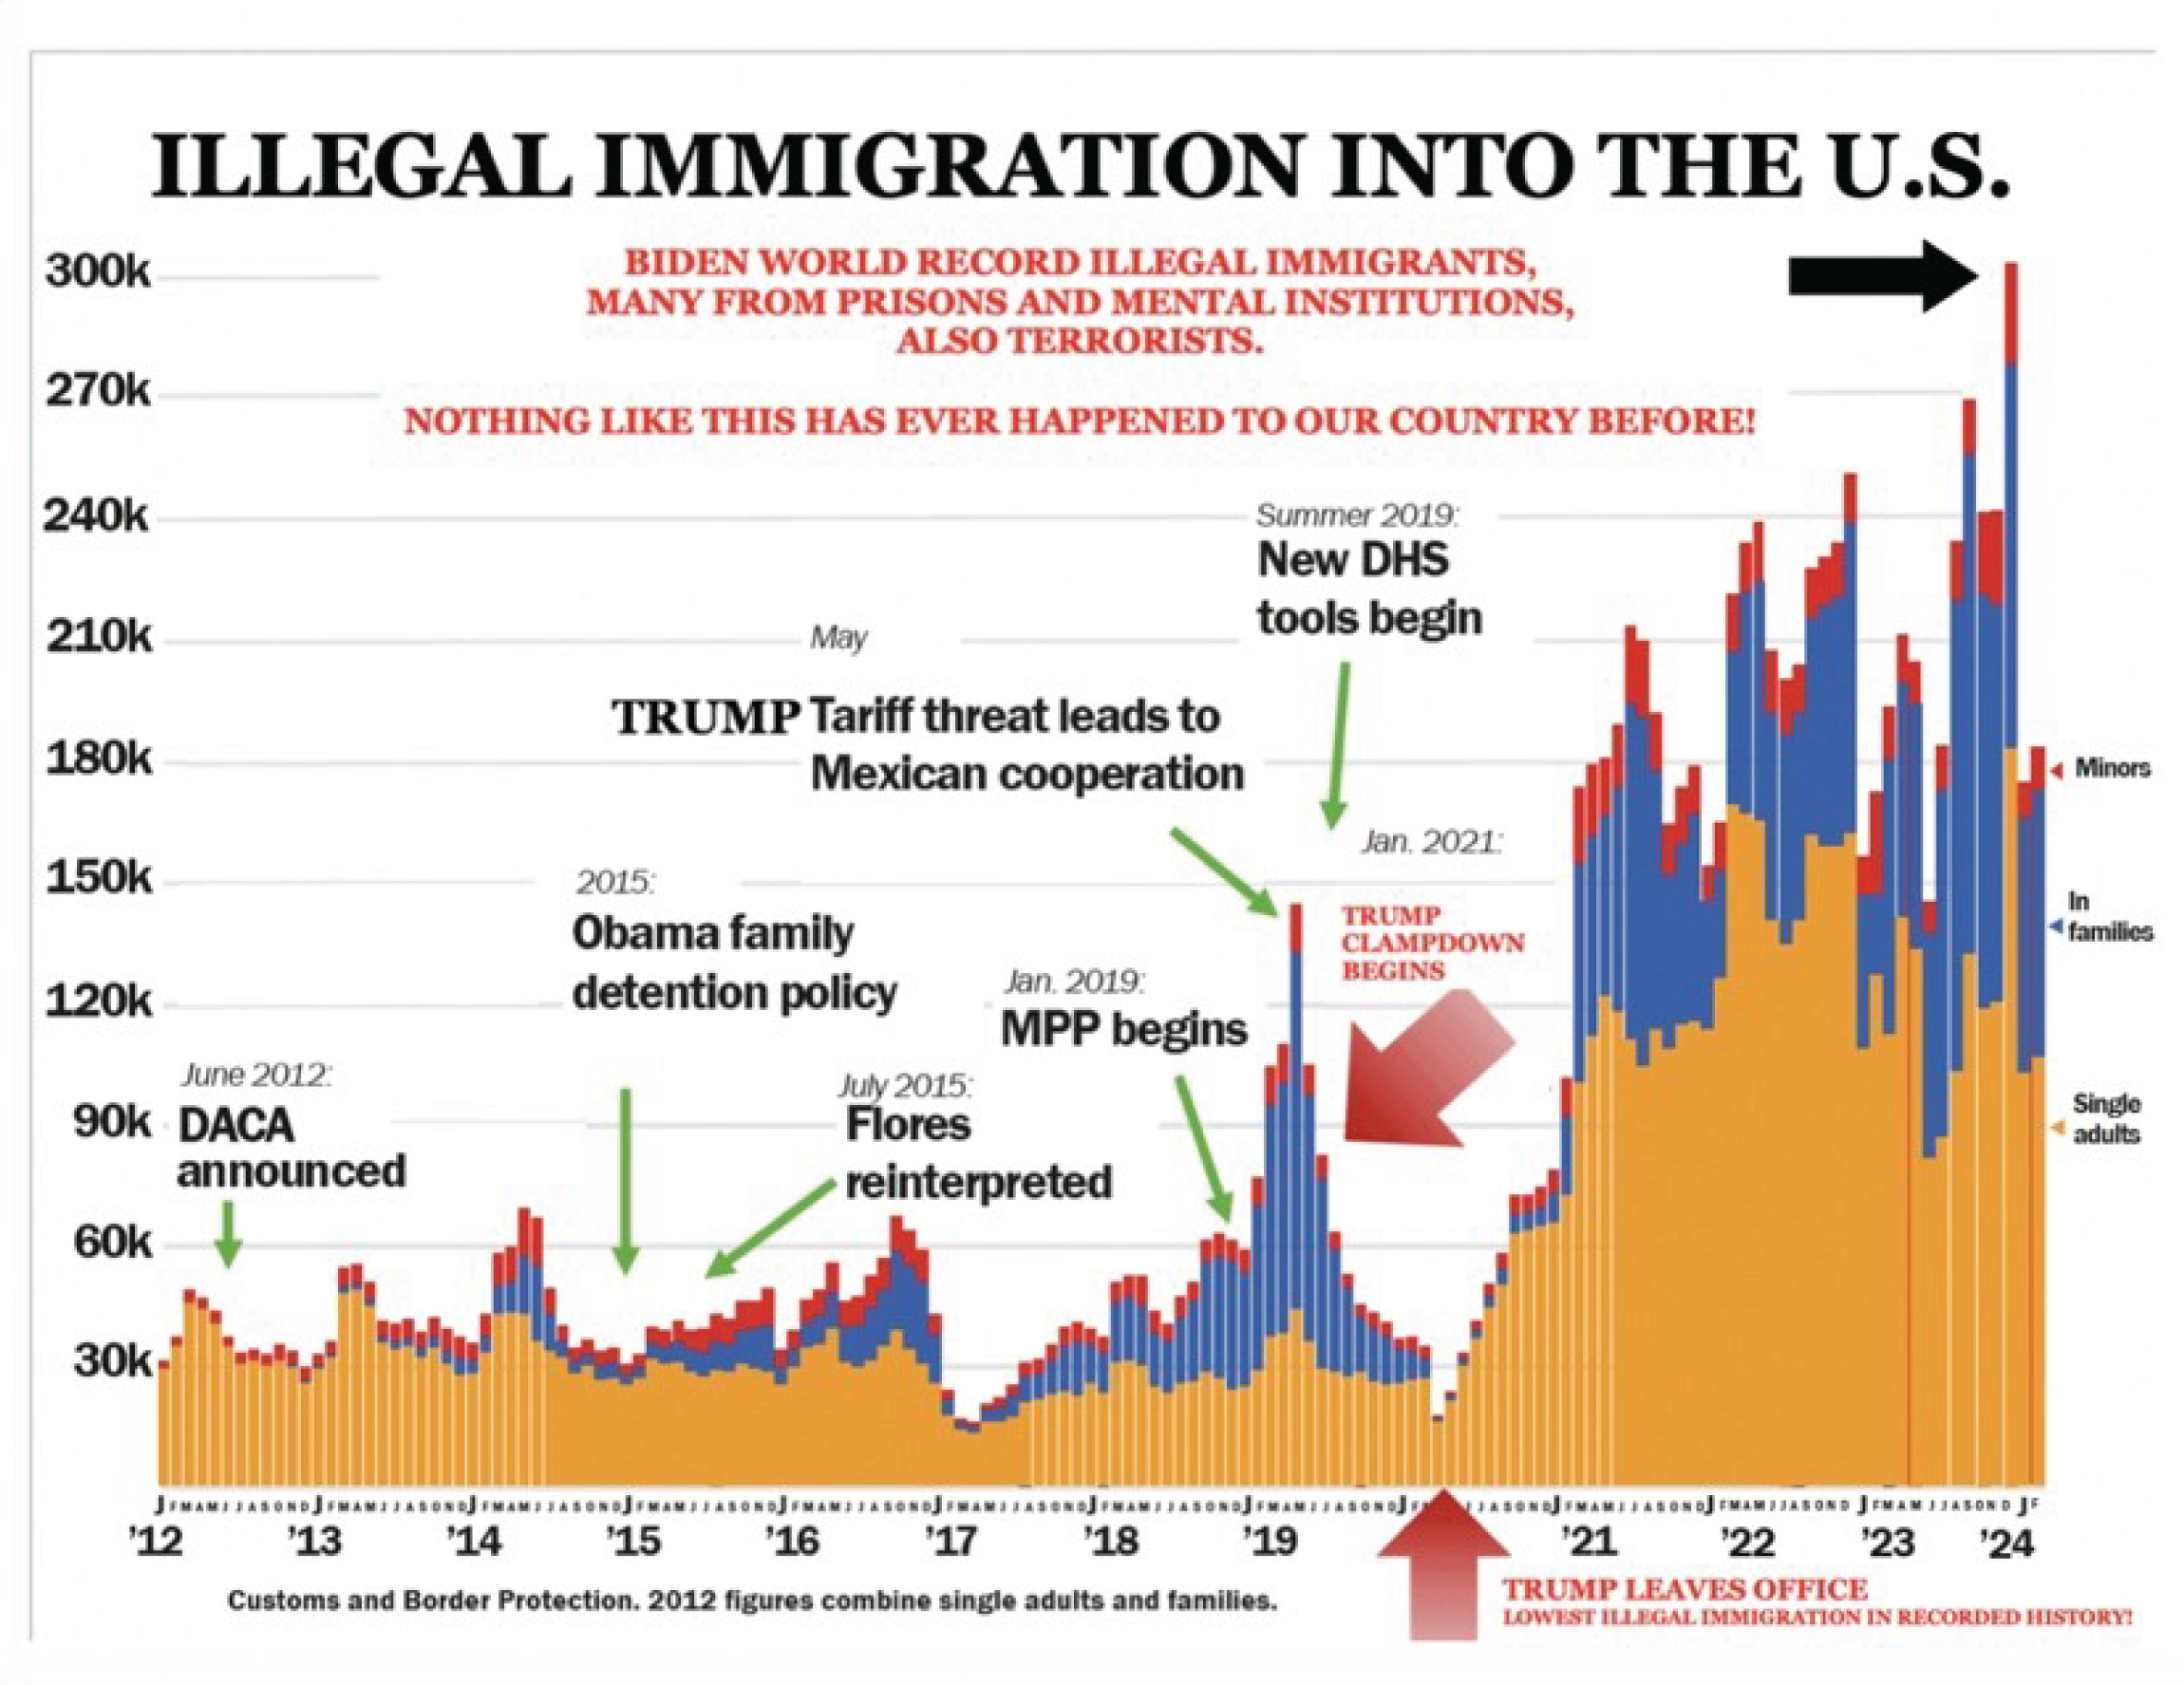
\includegraphics[width=0.75\textwidth]{figs/Trump Chart.png}
%   \caption{
%       Trump's Illegal Immigration Chart
%   }
%   \label{fig:fig1}
% \end{figure}




\begin{refcontext}[sorting=nyt]
\printbibliography
\end{refcontext}

\end{document}

